\chapter{Deformed Nuclei}

\section{Nuclear deformation}

Most of the nuclei across the nuclide chart are spherical or symmetric in their ground state. Moreover, for the axially symmetric nuclei (i.e, either \emph{oblate} or \emph{prolate}), there is a prolate over oblate dominance.
% \begin{figure}[ht]
%     \centering
%     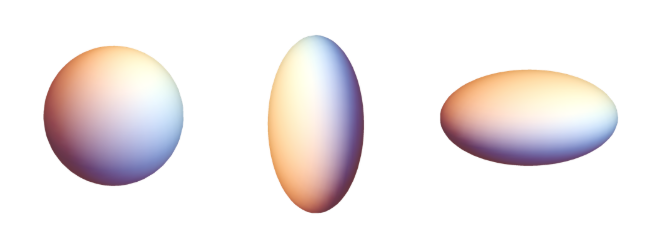
\includegraphics[scale=0.3]{Chapters/Figures/nuclear_shapes.png}
%     \caption{Nuclear Shapes.}
%     \label{nuclear_shapes}
% \end{figure}

The spherical shell model only describes nuclei near the closed shells. On the other side, for the nuclei that lie far from closed shells, a deformed potential must be employed. 
\par In the case of even-even nuclei, unique band structures resulting from the vibrations and rotations of the nuclear surface (as proposed by Bohr and Mottelson \cite{bohr1998nuclear} in the \emph{Geometric Collective Model} - GCM) appear in the energy range 0-2 MeV.

Within the GCM, the nucleus is described as a classical charged liquid drop. For the low-lying energy spectrum, usually, the compression of nuclear matter and the nuclear skin thickness are neglected. This results in the final picture of a liquid drop with a constant nuclear density and a sharp surface \cite{greiner1996nuclear}.

\subsection{Collective coordinates}

The nuclear surface can be described via an expansion of the spherical harmonic functions with some time-dependent parameters as \emph{expansion coefficients}. The expression of the nuclear shape is shown below \cite{greiner1996nuclear}:
\begin{align}
    R(\theta,\varphi,t)=R_0\left(1+\sum_{\lambda=0}^\infty\sum_{-\lambda}^\lambda\alpha_{\lambda\mu}(t)Y_\lambda^\nu(\theta,\varphi)\right)\ .
    \label{nuclear-shape}
\end{align}

In \ref{nuclear-shape}, $R$ denotes the nuclear radius as a function of the spherical coordinates $\theta,\varphi)$ expressing the direction, and the time $t$, while $R_0$ is the radius of the spherical nucleus when all the expansion coefficients vanish. It is worth mentioning that the expansion coefficients $\alpha_{\lambda\mu}$ act as \emph{collective coordinates} since the time-dependent amplitudes describe the vibrations of the nuclear surface.

\subsection{Nuclear radius under rotation}

To get a grasp at the physical meaning behind the deformation parameters that are used to describe the nuclear surface, it is instructive to see what happens when the system undergoes a rotation transformation.

The function $R(\theta,\varphi)$ describes the original (non-rotated) nuclear shape. Rotating the system will result in the change of the angular coordinates $(\theta,\varphi)$ to $(\theta',\varphi')$, which will correspond to a new function $R'(\theta',\varphi')$. Moreover, both nuclear surfaces (i.e., the non-rotated and the rotated one) must hold the equality:
\begin{align}
    R'(\theta',\varphi')=R(\theta,\varphi)
\end{align}

The rotational invariance of $R$ employs that $R'(\theta,\varphi)$ must have the same functional form, but the expansion coefficients $\alpha_{\lambda\mu}$ must be rotated, meaning:
\begin{align}
    \sum_{\lambda\mu}\alpha_{\lambda\mu}'Y'_{\lambda\mu}(
        \theta,\varphi)=\sum_{\lambda\mu}\alpha_{\lambda\mu}Y_{\lambda\mu}(
            \theta,\varphi)\ . \label{nuclear_surface_equality}
\end{align}

Note that in Eq. \ref{nuclear_surface_equality}, the spherical harmonics $Y'_{\lambda\mu}$ are obtained via the usual rotation matrices. Finally, the invariance of Eq. \ref{nuclear-shape} is achieved if the set of parameters $\alpha_{\lambda\mu}$ transform similarly to a \emph{spherical tensor with angular momentum} $\lambda$ \cite{ring2004nuclear}, that is:
\begin{align}
    \alpha_{\lambda\mu}'=\sum_{\mu'}\mathcal{D}^{(\lambda)}_{\mu\mu'}\alpha_{\lambda\mu'}\ .
\end{align}

Besides the spherical tensor character, the collective coordinates also have the following properties (emerging from Eq. \ref{nuclear-shape}):
\begin{itemize}
    \item Complex Conjugation.
    \begin{align}
        Y^*_{\lambda\mu}(\theta,\varphi)&=(-1)^{\mu}Y_{\lambda-\mu}(\theta,\varphi), \\
        \alpha^*_{\lambda\mu}&=(-1)^\mu\alpha_{\lambda-\mu}\ .
    \end{align}
    \item Parity - the coordinates $\alpha_{\lambda\mu}$ must undergo the same change of sign under a parity transformation as the spherical harmonics, in order to keep the invariance of the nuclear surface.
    \begin{align}
        (r,\theta,\varphi) &\xrightarrow[P]{}     (r,\pi-\theta,\pi+\varphi)\ \nonumber, \\
        Y_{\lambda\mu}(\theta,\varphi) &\xrightarrow[P]{} Y_{\lambda\mu}(\pi-\theta,\pi+\varphi)=(-1)^\lambda Y_{\lambda\mu}(\theta,\varphi)\ .\nonumber
    \end{align}
    Therefore, the parity of the expansion coefficients are:
    \begin{align}
        \pi(\alpha_{\lambda\mu})=(-1)^\lambda\ .
    \end{align}
\end{itemize}

\subsection{Multipole deformations}

In the expansion of the nuclear surface defined by Eq. 
\ref{nuclear-shape}, the different values for $\lambda$ will determine different effects regarding the physical aspects of the nucleus. As such, the first values of $\lambda$ will be examined in terms of the physical meaning.

\begin{description}
    \item[Monopole mode] This corresponds to the first value of $\lambda=0$. This is the simplest mode of \emph{deformation} of a nuclear surface. Within this approximation, the spherical harmonic $Y_0^0$ is constant, which would imply that any non-vanishing values for $\alpha_{00}$ will correspond to the change in radius of the nucleus. This kind of excitation is also called \emph{breathing mode} of the nucleus \cite{greiner1996nuclear,bohr1998nuclear}. The energy required for this kind of excitation mode is very large, since it implies a compression of the nuclear matter. As a result, this mode is irrelevant in the low-lying excited spectra of atomic nuclei.
\end{description}